%!TEX program =pdflatex
\documentclass{beamer}
\usetheme{CambridgeUS}
\author{J.J. Cai, J.H.J Einmahl, L. de Haan 
and C. Zhou}
\date{}

%%define new comand
\def\argmin{\mathop{\rm arg~min}\limits}
\newcommand{\suit}[1]{\left(#1\right)}
\newcommand{\abs}[1]{\left\vert#1\right\vert}
\newcommand{\set}[1]{\left\{#1\right\}}
\newcommand{\bra}[1]{\left[ #1 \right]}
\title{Estimation of the marginal expected shortfall: the
mean when a related variable is extreme}
\begin{document}
\begin{frame}
\titlepage
\vspace{-10ex}
\begin{center}
    Published on J.R. Statist. Soc. B (2015).

    \vspace{3ex}
\end{center}
\end{frame}

\AtBeginSection[]
{
    \begin{frame}
        \frametitle{Table of Contents}
        \tableofcontents[currentsection]
    \end{frame}
}

\section{Introduction}
\begin{frame}
    \frametitle{Expected shortfall}
We use capital letter to denote the loss of an asset.

    \bigskip
    Expected shortfall of an asset $X$ at probability level $p$ is defined as 
    $$
      E\suit{X|X\ge Q_{X}(1-p)}
    $$
where
$$
F_X(x) = P\suit{X\le x}
$$
and $Q_{X}$ denotes the inverse function of $F_X$.
    

\end{frame}


\begin{frame}
    \frametitle{Marginal Expected Shortfall (MES)}
\begin{itemize}
    \item A financial institute holds a portfolio $R = \sum_{i} y_i R_i$
    \item Expected shortfall at probability level $p$
    $$
      E\suit{R|R>Q_R(1-p)}
    $$
    \item Can be decomposed as 
    $$
        \sum_{i} y_i E\suit{{\color{blue} R_i}|R>Q_{R}(1-p)}
    $$
    \item The sensitivity to the i-th asset is
    $$
    E\suit{R_i|R>Q_{p}(1-p)}.
    $$
\end{itemize}
    

\end{frame}

\begin{frame}
    \frametitle{MES}
    \begin{itemize}
        \item Marginal expectation shortfall is also often used to measure the contribution of a financial institute to a systemic crisis.
        \medskip

        \item It is defined as  an institute' s expected equity loss when market falls below a certain threshold.
        
        \medskip
        \item "$R_i$": a particular finiancial institute, "$R$": the total market. 
    \end{itemize}
    

\end{frame}

\begin{frame}
    \frametitle{MES}

\begin{itemize}
    \item More generally: consider a random vector $(X,Y)$
    \vspace{5ex}
    \item Marginal expected shortfall (MES) of $X$ at level $p$ is 
    $$
    E\suit{X|Y>Q_Y(1-p)}
    $$
\end{itemize}

\end{frame}


\begin{frame}
    \frametitle{MES}
\begin{itemize}
    \item In this paper, we are interested in MES under exceptional stress
    conditions of the kind that have occurred very
    rarely or even not at all.  ($p$ is at an
    extremely low level that can be even lower than $1/n$)

    \vspace{5ex}
    \item We assume that $p=p_n\to 0$, (intermediate level) $np_n \to\infty$,  and (extreme level) $np_n = O(1)$ as $n\to \infty$.   
    \vspace{5ex}
   \item We want to estimate $E\suit{X|Y>Q_Y(1-p)}$
   for small $p$ on the basis of i.i.d. observations
   $$
        (X_1,Y_1),(X_2,Y_2,),\dots,(X_n,Y_n)
   $$
\end{itemize}
    

\end{frame}



\section{Main Results}
\begin{frame}
    \frametitle{Notations}
$$
U_1(t) =Q_X\suit{1-\frac{1}{t}} =F_X^{\leftarrow}\suit{1-\frac{1}{t}}
$$
$$
U_2(t) =Q_Y\suit{1-\frac{1}{t}}
$$
$$
\theta_p = E\suit{X|Y>U_2\suit{\frac{1}{p}}}
$$
    

\end{frame}



\begin{frame}
    \frametitle{}
    For the time being we suppose that $X>0$.
    $$
\begin{aligned}
    \theta_p &= E\suit{X|Y>U_2\suit{\frac{1}{p}}} \\
    &= \frac{\int_{0}^{\infty}P\set{X>x,Y>U_2\suit{\frac{1}{p}}}dx}{{\color{blue}P\set{Y>U_2\suit{\frac{1}{p}}}}}  \\ 
    &={\color{blue}\frac{1}{p}}\int_{0}^{\infty} P\set{X>x, Y>U_2\suit{\frac{1}{p}}} dx\\
    &=\frac{1}{p}U_1\suit{\frac{1}{p}}\int_0^{\infty} P\set{X>x U_1\suit{\frac{1}{p}}, Y>U_2\suit{\frac{1}{p}}}dx.
\end{aligned}
$$
    
Thus,
$$
\frac{\theta_p}{U_1\suit{\frac{1}{p}}} = \frac{1}{p}\int_0^{\infty} P\set{X>x U_1\suit{\frac{1}{p}}, Y>U_2\suit{\frac{1}{p}}}dx.
$$

\end{frame}


\begin{frame}
    \frametitle{Condition (1)}


 First note (take $x=1$ upstairs)
$$
\begin{aligned}
&P\set{X>U_1\suit{\frac{1}{p}},Y>U_2\suit{\frac{1}{p}}}\\
&=P\set{1-F_1(X)<p,1-F_2(Y)<p}.
\end{aligned}
$$

\vspace{5ex}

This is a copula.
\end{frame}


\begin{frame}
    \frametitle{Condition (1)}
We impose conditions on the copula as $p\to 0$.
\medskip

Suppose there exists a positive function $R(x,y)$ such that for all
$$
0\le x,y\le \infty, x\lor y>0, x\wedge y<\infty
$$

$$
\lim_{p\to 0} \frac{1}{p} P\set{X>U_1\suit{\frac{1}{xp}}, Y>U_2\suit{\frac{1}{yp}}} = R(x,y).
$$
i.e.,
$$
\lim_{p\to 0} \frac{1}{p} P\set{1-F_1(X)<px, 1-F_2(Y)<py} = R(x,y).
$$
    
This condition indicates and specifies {\color{blue} dependence  in the tail.}  ( usual condition in extreme value theory)
\end{frame}


\begin{frame}
    \frametitle{Condition (2)}
    Compare: in the definition of $\theta_p$ we have
    $$
P\set{X>{\color{blue} x}U_1\suit{\frac{1}{p}}, Y>U_2\suit{\frac{1}{p}}}
    $$
and in the condition we have (for $y=1$)
$$
P\set{X>U_1\suit{\frac{ 1}{{\color{blue} x} p}}, Y>U_2\suit{\frac{1}{p}}}.
    $$
\end{frame}

\begin{frame}
    \frametitle{Condition (2)}
    In order to connect the two we impose a second
    condition, on the $U$ : for $x>0$
    $$
    \lim_{t\to \infty} \frac{U_1(tx)}{U_1(t)} = x^{\gamma_1}, \quad x>0.
    $$
where $\gamma_1>0$. 


\end{frame}



\begin{frame}
    \frametitle{Proposition 1}
Under these conditions, we get the first result:

$$
\lim_{p\to 0} \frac{\theta_p}{U_1\suit{\frac{1}{p}}} = \lim_{p\to 0} \frac{E\suit{X|Y>U_2\suit{\frac{1}{p}}}}{U_1\suit{\frac{1}{p}}} = \int_0^{\infty} R(x^{-1/\gamma_1},1)dx.
$$

\medskip

Hence, $\theta_p$ goes to infinity as $p\to 0$ as the same rate as $U_1\suit{\frac{1}{p}}$, the value at risk for $X$.

\end{frame}


\begin{frame}
    \frametitle{Estimation for $\theta_p$.}
    Now we go to statistics and look at how to
    estimate $\theta_p$.

    Wo do that in stages:
    \begin{itemize}
        \item First, we estimate $\theta_{k/n}$ where $ k =k(n)\to\infty, k/n \to 0$ as $n \to \infty$.
        
        We can estimate $\theta_{k/n}$ non-parametrically.

        \item The second stage will be the extrapolation from $\theta_{k/n}$ to $\theta_p$ with $np_n=O(1)$.
    \end{itemize}

    

\end{frame}

\begin{frame}
    \frametitle{Estimation for $\theta_{k/n}$.}

Recall $\theta_{k/n} =E\suit{X|Y>U_2\suit{\frac{n}{k}}}$

\begin{itemize}
    \item Replace quantile $U_2(n/k)$ by corresponding sample quantile $Y_{n-k,n}$ ($k$-th order statistics from above)
    \item Replace the expectation by the sample mean.

\end{itemize}

The obvious estimation of $\theta_{k/n}$ is then 
$$
\hat{\theta}_{k/n}:= \frac{\frac{1}{n}\sum_{i=1}^n X_i 1_{\set{Y_i>Y_{n-k,n}}}}{P\suit{Y>U_2\suit{\frac{n}{k}}}} = \frac{1}{k}\sum_{i=1}^n X_i 1_{\set{Y_i>Y_{n-k,n}}}
$$
\end{frame}


\begin{frame}
    Under some strengthening of our conditions (relating to $R$ and to the sequences $k(n)$),
    $$
\sqrt{k}\suit{\frac{\hat{\theta}_{k/n}}{\theta_{k/n}}-1} \stackrel{d}{\to} \Theta,
    $$
 a normal random variable that we describe now.

 Background of limit result is the assumption
$$
\lim_{p\to 0} \frac{1}{p} P\suit{1-F_1(X)<px,1-F_2(Y)<py} = R(x,y).
$$

Now define $V:=1-F_1(X)$

\quad \quad \quad \quad \quad $W:=1-F_2(Y).$

$V$ and $W$ have a uniform distribution, their joint distribution is a copula.
\end{frame}

\begin{frame}
    \frametitle{Tail Copula}
    \begin{itemize}
        \item     Now consider the i.i.d. r.v.'s
        $$
            (V_i,W_i) = (1-F_1(X_i),1-F_2(Y_i)) \quad (i\le n)
        $$
        \item Empirical distribution function: $\frac{1}{n}\sum_{i=1}^n 1_{\set{V_i\le x,W_i\le y}}$.
        \item We consider the left tail of $(V_i,W_i)$ i.e., the right tail for $(X_i,Y_i)$.
        \item We define the tail version 
        $$
            T_n(x,y):=\frac{1}{k}\sum_{i=1}^n 1_{\set{V_i\le {\color{blue}\frac{kx}{n}},W_i\le {\color{blue}\frac{ky}{n}}}}.
        $$
    \end{itemize}

    

\end{frame}

\begin{frame}
    \frametitle{Tail Copula}
Now, $T_n(x,y)$ is close to its mean which is
$$
\frac{n}{k}P\set{1-F_1(X)\le \frac{kx}{n},1-F_2(Y)\le \frac{ky}{n}}
$$
and this is close  to $R(x,y)$ (as $n\to \infty$.)

"Hence" $T_n(x,y)\stackrel{P}{\to} R(x,y)$ and 
$$
\sqrt{k}\suit{T_n(X,Y)-R(x,y)}
$$
converges in distribution to a mean zero Gaussian
process  $W_R$.

This stochastic process $W_R(x,y)$ has independent
increments that is,
$$
E W_R(x_1,y_1)W_R(x_2,y_2) =R(x_1\vee x_2, y_1 \vee y_2).
$$
\end{frame}


\begin{frame}
    \frametitle{Convergence for $\hat{\theta}_{k/n}$}
$$
\begin{aligned}
\int_0^{\infty} T_n(x,1) dx^{-\gamma_1} =&\frac{1}{k}\sum_{i=1}^n \int_0^{\infty} 1_{\set{X_i>U_1\suit{\frac{n}{k{\color{red} x}}},Y_i>U_2\suit{\frac{n}{k}}}} dx^{-\gamma_1} \\
\stackrel{U_1\in R.V.}{\approx}& \frac{1}{k}\sum_{i=1}^n \int_0^{\infty} 1_{\set{X_i>{\color{red}x^{-\gamma_1}}U_1\suit{\frac{n}{k}},Y_i>U_2\suit{\frac{n}{k}}}} dx^{-\gamma_1} \\
=&\frac{1}{k}\sum_{i=1}^n \int_0^{\infty} 1_{\set{X_i>xU_1\suit{\frac{n}{k}},Y_i>U_2\suit{\frac{n}{k}}}} dx \\
=&\frac{1}{k}\sum_{i=1}^n \int_0^{\infty} 1_{\set{X_i>xU_1\suit{\frac{n}{k}}}} 1_{\set{Y_i>U_2\suit{\frac{n}{k}}}} dx
\end{aligned}
$$  

\end{frame}

\begin{frame}
    \frametitle{Cont.}
$$
\begin{aligned}
=&\frac{1}{k}\sum_{i=1}^n 1_{\set{Y_i>U_2\suit{\frac{n}{k}}}} \int_0^{X_i/U_1(n/k)}dx \\
=&\frac{1}{k}\sum_{i=1}^n \frac{X_i}{U_1\suit{\frac{n}{k}}}1_{\set{Y_i>{\color{blue} U_2\suit{\frac{n}{k}}}}} \\
\approx& \frac{1}{k}\sum_{i=1}^n \frac{X_i}{U_1\suit{\frac{n}{k}}}1_{\set{Y_i>{\color{blue} Y_{n-k,n}}}} =\frac{\hat{\theta}_{k/n}}{U_1(n/k)}. 
\end{aligned}
$$
    

\end{frame}

\begin{frame}
    \frametitle{Cont.}
Hence,
$$
\frac{\sqrt{k}}{U_1(n/k)}\suit{\hat{\theta}_{k/n}-\theta_{k/n}}\approx \sqrt{k}\int_0^{\infty} \set{T_n(x,1)-R(x,1)}dx^{-1/\gamma}
$$
and we get that
$$
\begin{aligned}
&\sqrt{k}\set{\frac{\hat{\theta}_{k/n}}{\theta_{k/n}}-1}\\
& \stackrel{d}{\to} (\gamma_1-1)W_R(\infty,1)+\suit{\int_0^{\infty} R(s,1)ds^{-\gamma
_1}}^{-1}\int_{0}^{\infty} W_R(s,1)ds^{-\gamma_1}
\end{aligned}
$$

\end{frame}


\begin{frame}
    \frametitle{Extrapolation}
\begin{itemize}
    \item We need to extrapolate from $\theta_{k/n}$ to $\theta_p$.
    \item Consider our first (non-statistical) result again:
    $$
\lim_{p\to 0}\frac{E\suit{X|Y>U_2(1/p)}}{U_1(1/p)} = \int_0^{\infty} R(x^{-1/\gamma_1},1)dx
    $$
\item In particular this holds for $p=k/n$, i.e,
$$
\lim_{n\to \infty}\frac{E\suit{X|Y>U_2(n/k)}}{U_1(n/k)} = \int_0^{\infty} R(x^{-1/\gamma_1},1)dx
$$
\item Thus, we have that, for suffiently large $n$,
$$
\frac{\theta_p}{U_1(1/p)} \approx \frac{\theta_{k/n}}{U_1(n/k)}.
$$
\end{itemize}
\end{frame}


\begin{frame}
    \frametitle{Extrapolation}
We have that,
$$
\begin{aligned}
    \theta_p & = E\suit{X|Y>U_2(1/p)} \\
    &\sim \frac{U_1(1/p)}{U_1(n/k)} E\suit{X|Y>U_2(n/k)}\\
    &=\frac{U_1(1/p)}{U_1(n/k)}\theta_{k/n}
\end{aligned}
$$
 This leads to an estimate for $\theta_p$
 $$
 \hat{\theta}_p =\frac{\widehat{U_1(1/p)}}{\widehat{U_1(n/k)}}\hat{\theta}_{k/n}
 $$
Here, $\hat{\theta}_{k/n}$ is the estimator we discussed before and $\widehat{U_1(n/k)}=X_{n-k,n}$.
\end{frame}


\begin{frame}
    \frametitle{Estimation for $\widehat{U_1(1/p)}$ }
    \begin{itemize}
        \item It remains to define and
        to study $\widehat{U_1(1/p)}$ with $np_n=O(1)$.
        \item Now, $U_1(1/p)$ is a one-dimensional object.
        \item Recall the condition $ U\in RV$, i.e., 
        $$
            \lim_{t\to \infty} \frac{U_1(tx)}{U_1(t)} =x^{\gamma_1}.
        $$
        \item Hence, for large $t$, $U_1(tx)\approx x^{\gamma_1} U_1(t)$
        \item Use this relation with $t:=n/k, tx=1/p$, we get 
        $$
            U_1(1/p)\approx U_1(n/k)\suit{\frac{k}{np_n}}^{\gamma_1}.
        $$
        \item This suggests the estimator for $\widehat{U_1(1/p)}$:
        $$
        \widehat{U_1(1/p)}=X_{n-k,n}\suit{\frac{k}{np_n}}^{\hat{\gamma}_1}.
        $$
    \end{itemize}
    
    

\end{frame}

\begin{frame}
    \frametitle{Estimation for $\gamma_1$}
\begin{itemize}
    \item Since $\gamma_1>0$, we use the well-known Hill estimator:
    $$
        \hat{\gamma}_1 =\frac{1}{k_1} \sum_{i=1}^{k_1-1} \log X_{n-i,n}-\log X_{n-k_1,n} 
    $$
    \item $k_1$ may differ from $k$ but satisfies similar conditions.
    \item Property of Hill's estimator:
    $$
        \sqrt{k_1}\suit{\hat{\gamma}_1-\gamma_1}\stackrel{d}{\to}\Gamma
    $$
\end{itemize}
    
\end{frame}
\begin{frame}
    \frametitle{Property of $\widehat{U_1(1/p)}$}
\begin{itemize}
    \item Property of $X_{n-k,n}$
    $$
\sqrt{k}\suit{\frac{X_{n-k,n}}{U_1(n/k)}-1}\stackrel{d}{\to} N_0
    $$
    \item Combine the two relations:
    $$
    \begin{aligned}
        \frac{\widehat{U_1(1/p)}}{U_1(1/p)} &= \frac{X_{n-k,n}}{U_1(n/k)}{\color{blue}\frac{U_1(n/k)}{U_1(1/p_n)}}\suit{\frac{k}{np_n}}^{\hat{\gamma}_1} \\
        &\approx \frac{X_{n-k,n}}{U_1(n/k)} {\color{blue}\suit{\frac{np_n}{k}}^{\gamma_1}}\suit{\frac{k}{np_n}}^{\hat{\gamma}_1}\\
        &=\frac{X_{n-k,n}}{U_1(n/k_1)} \suit{\frac{k}{np_n}}^{\hat{\gamma}_1-\gamma_1}
    \end{aligned}
    $$
\end{itemize}
    

\end{frame}

\begin{frame}
    \frametitle{Cont.}

$$
\begin{aligned}
    & \approx \suit{1+\frac{N_0}{\sqrt{k}}}\exp\set{\sqrt{k_1}\suit{\hat{\gamma_1}-\gamma_1}\frac{\log \frac{k}{np_n}}{\sqrt{k_1}}}.
\end{aligned}
$$
\begin{itemize}
    \item Now, assume that 
    $$
    \frac{\log \frac{k}{np_n}}{\sqrt{k_1}} \to 0,
    $$
    (this means that $p$ can not be too small.)
    \item Then (expansion of function “exp”)
    $$
    \frac{\widehat{U_1(1/p)}}{U_1(1/p)} \approx \suit{1+\frac{N_0}{\sqrt{k}}}\set{1+\sqrt{k_1}\suit{\hat{\gamma_1}-\gamma_1}\frac{\log \frac{k}{np_n}}{\sqrt{k_1}}}
    $$
\end{itemize}
\end{frame}


\begin{frame}
    \frametitle{Cont.}
Hence,
$$
\frac{\sqrt{k_1}}{\log\frac{k}{np_n} }\suit{\frac{\widehat{U_1(1/p)}}{U_1(1/p)} -1}\stackrel{d}{\to} \Gamma
$$
\end{frame}
 
% \begin{frame}
%     \frametitle{Conditions:}
% \begin{itemize}
%     \item There exist $\beta>\gamma_1$ and $\tau<0$ such that, as $t\to \infty$,
%     $$
%     \sup _{0<x<\infty \atop 1 / 2 \leqslant y \leqslant 2} \frac{\left|t P\left\{1-F_{1}(X)<x / t, 1-F_{2}(Y)<y / t\right\}-R(x, y)\right|}{x^{\beta} \wedge 1}=O\left(t^{\tau}\right)
%     $$
%     \item There exists $\rho_1<0$ and an eventually positive or negative function $A_1$ such that, as $t\to \infty$, $A_1(tx)/A_1(t)\to x^{\rho_1}$ for all $x>0$ and
%     $$
%     \sup _{x>1}\left|x^{-\gamma_{1}} \frac{U_{1}(t x)}{U_{1}(t)}-1\right|=O\left\{A_{1}(t)\right\}
%     $$
%     \item $\sqrt{k_1}A_1\suit{n/k_1}\to 0$.
%     \item $k=O(n^{\alpha})$ for some $\alpha<\min\suit{\frac{-2\tau}{-2\tau+1},\frac{2\gamma_1\rho_1}{2\gamma_1\rho_1+\rho_1-1}}$
% \end{itemize}
% \end{frame}

\begin{frame}
    \frametitle{Theorem 1}


{\bf Technical Conditions}:
\begin{itemize}
    \item[(a)] There exists $\beta>\gamma_1$ and $\tau<0$ such that as $t\to\infty$,
    $$
    \sup _{0<x<\infty \atop 1 / 2 \leqslant y \leqslant 2} \frac{\left|t P\left\{1-F_{1}(X)<x / t, 1-F_{2}(Y)<y / t\right\}-R(x, y)\right|}{x^{\beta} \wedge 1}=O\left(t^{\tau}\right)
    $$ 
    \item[(b)] There exist $\rho_1<0$ and $A_1\in RV(\rho_1)$, such that 
    $$
        \sup_{x>1}\abs{x^{-\gamma_1}\frac{U_1(tx)}{U_1(t)}-1} =O\set{A_1(t)}.
    $$
    \item[(c)] As $n\to\infty$, $\sqrt{k_1}A(n/k_1) \to 0$.
    \item[(d)] As $k\to \infty$, $k=O(n^{\alpha})$ for some $\alpha <\min\set{-2\tau/(-2\tau+1),2\gamma_1\rho_1/(2\gamma_1\rho_1+\rho_1-1)}$ 
\end{itemize}
\end{frame}

\begin{frame}
    \frametitle{Theorem 1}

    \begin{itemize}
        \item Suppose the conditions (a)-(d) hold.
        \item Suppose $\gamma\in(0,1/2)$.
        \item  Suppose $X>0$.
        \item Assume $d_n = \frac{k}{np_n}\ge 1$ and $\log d_n/\sqrt{k_1}\to 0$.
      
    \end{itemize}
    Denote $r = \lim_{n\to \infty} \frac{\sqrt{k}\log d_n}{\sqrt{k_1}}\in [0,\infty]$. Then, as $n\to \infty$,
    $$
    \min\suit{\sqrt{k},\frac{\sqrt{k_1}}{\log d_n}}\suit{\frac{\hat{\theta}_p}{\theta_p}-1}\stackrel{d}{\to} \left\{
        \begin{array}{c}
            \Theta+r\Gamma, \ \text{if}\  r\le 1, \\
            \frac{1}{r}\Theta+\Gamma, \ \text{if} \ r>1.
        \end{array}
     \right.
    $$  

\end{frame}
\begin{frame}
    \frametitle{$X$ real}
    So far we assumed $X>0$.

    For general $X\in \mathbb{R}$ we need some extra conditions
\begin{itemize}
    \item Thinner left tail: $E\abs{\min(X,0)}^{1/\gamma_1}<\infty$
    \item A further bound on $p=p_n$.
\end{itemize}
    
We estimate $\theta_p$ with 
$$
\suit{\frac{k}{np_n}}^{\hat{\gamma_1}}\frac{1}{k}\sum_{i=1}^n X_i I({\color{blue} X_i>0},Y_i>Y_{n-k,n})
$$

\end{frame}
\section{Simulation}

\begin{frame}
    \frametitle{Simulation Distributions}
\begin{itemize}
    \item Generate Data from three bivariate distributions.
    \bigskip
    \item     Let $(Z_1,Z_2)$ denotes a standard Cauchy distribution on $\mathbb{R}^2$ with density $(1/2\pi)(1+x^2+y^2)^{-3/2}$.
\end{itemize}

    

\end{frame}

\begin{frame}
    \frametitle{Simulation Distributions}

\begin{itemize}
    \item transformed Cauchy distribution on $(0,\infty)^2$ defined as
	$$
	(X,Y)=(|Z_1|^{2/5},|Z_2|).
	$$
	It follows that $\gamma_1=2/5$ and $R(x,y)=x+y-\sqrt{(x^2+y^2)}, x, y \ge 0.$

    \item a Student $t_3$ -distribution on $(0,\infty)^2$ with density
	$$
	f(x, y)=\frac{2}{\pi}\left(1+\frac{x^{2}+y^{2}}{3}\right)^{-5 / 2}, \quad x, y>0.
	$$
	We have $\gamma_1=1/3, R(x,y)=x+y-(x^{4/3}+1/2x^{2/3}y^{2/3}+y^{4/3})/\sqrt{(x^{2/3}+y^{2/3})}$.

\item  a transformed Cauchy distribution on the whole $\mathbb{R}^2$ defined as 
	$$
    \begin{aligned}
	(X, Y)=\left(Z_{1}^{2 / 5} I\left(Z_{1} \geqslant 0\right)+Z_{1}^{1 / 5} I\left(Z_{1}<0\right) \right., \\
    \left. Z_{2} I\left(Z_{1} \geqslant 0\right)+Z_{2}^{1 / 3} I\left(Z_{1}<0\right)\right).
    \end{aligned}
	$$
	We have $\gamma_1=2/5, R(x,y)=x/2+y-\sqrt{(x^2/4+y)}$.
    
\end{itemize}
\end{frame}

\begin{frame}
    \frametitle{Other Estimators}
Besides the estimator we propose, we construct two other estimators.
\begin{itemize}
    \item[1.]  For $np\ge 1$,  an empirical counterpart of $\theta_p$, given by
    $$
    \hat{\theta}_{\mathrm{emp}}=\frac{1}{\lfloor n p\rfloor} \sum_{i=1}^{n} X_{i} I\left(Y_{i}>Y_{n-\lfloor n p\rfloor, n}\right).
    $$
\end{itemize}
\end{frame}
\begin{frame}
    \frametitle{Other Estimators}

\begin{itemize}
    \item[2.] Recall the first result,
    $$
\lim_{p\to 0} \frac{\theta_p}{U_1\suit{\frac{1}{p}}} = \lim_{p\to 0} \frac{E\suit{X|Y>U_2\suit{\frac{1}{p}}}}{U_1\suit{\frac{1}{p}}} = \int_0^{\infty} R(x^{-1/\gamma_1},1)dx.
$$.
Estimate 
    $$
    \hat{R}(x, y)=\frac{1}{k} \sum_{i=1}^{n} I\left(X_{i}>X_{n-\lfloor k x\rfloor, n}, Y_{i}>Y_{n-\lfloor k y\rfloor, n}\right), \quad x, y \geqslant 0.
    $$
    and  $\hat{U}_{1}(1 / p)=d_{n}^{\hat{\gamma}_{1}} X_{n-k, n}$,  we define an
    alternative EVT estimator as
    $$
    \begin{aligned}
    \bar{\theta}_{p} &=-\hat{U}_{1}\left(\frac{1}{p}\right) \int_{0}^{\infty} \hat{R}(x, 1) \mathrm{d} x^{-\hat{\gamma}_{1}} \\
    &=d_{n}^{\hat{\gamma}_{1}} X_{n-k, n} \frac{1}{k} \sum_{i=1}^{n} I\left(Y_{i}>Y_{n-k, n}\right)\left\{\frac{n-\operatorname{rank}\left(X_{i}\right)+1}{k}\right\}^{-\hat{\gamma}_{1}}
    \end{aligned}.
    $$
\end{itemize}


\end{frame}

\begin{frame}
    \frametitle{Simulation Setting}
\begin{itemize}
    \item 500 samples from each distribution with sample sizes $n=500$ and $n=2000$.
    \item On the basis of each sample, we estimate $\theta_p$ for $p=1/500,1/5000$ or $1/10000$.
\end{itemize}
    

\end{frame}

\begin{frame}
    \frametitle{Boxplot of the estimates}
    \begin{itemize}
        \item Transformed Cauchy distribution 1.
        \item $n=500, k=75, k_1 = 75, p_1=1/500, p_2=1/5000,p_3=1/10000$
    \end{itemize}

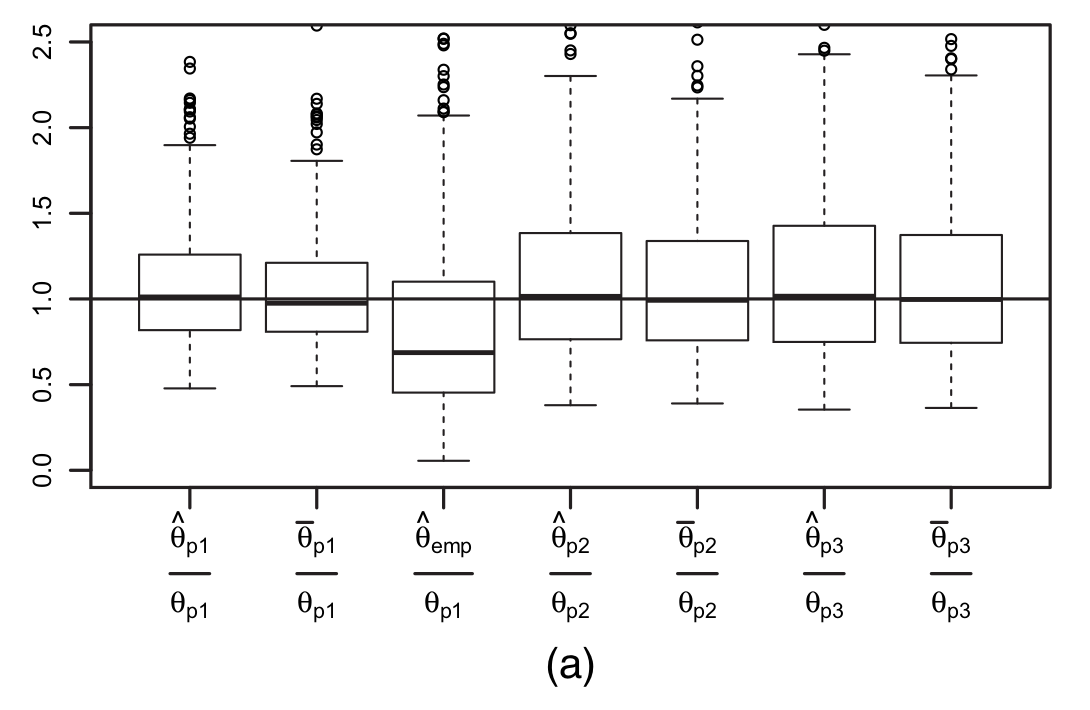
\includegraphics[width=0.8\textwidth]{a.png}
    

\end{frame}

\begin{frame}
    \frametitle{Boxplots of the estimates}
\begin{itemize}
    \item Student $t_3$ distribution
    \item $n=500, k=75, k_1 = 75, p_1=1/500, p_2=1/5000,p_3=1/10000$
\end{itemize}
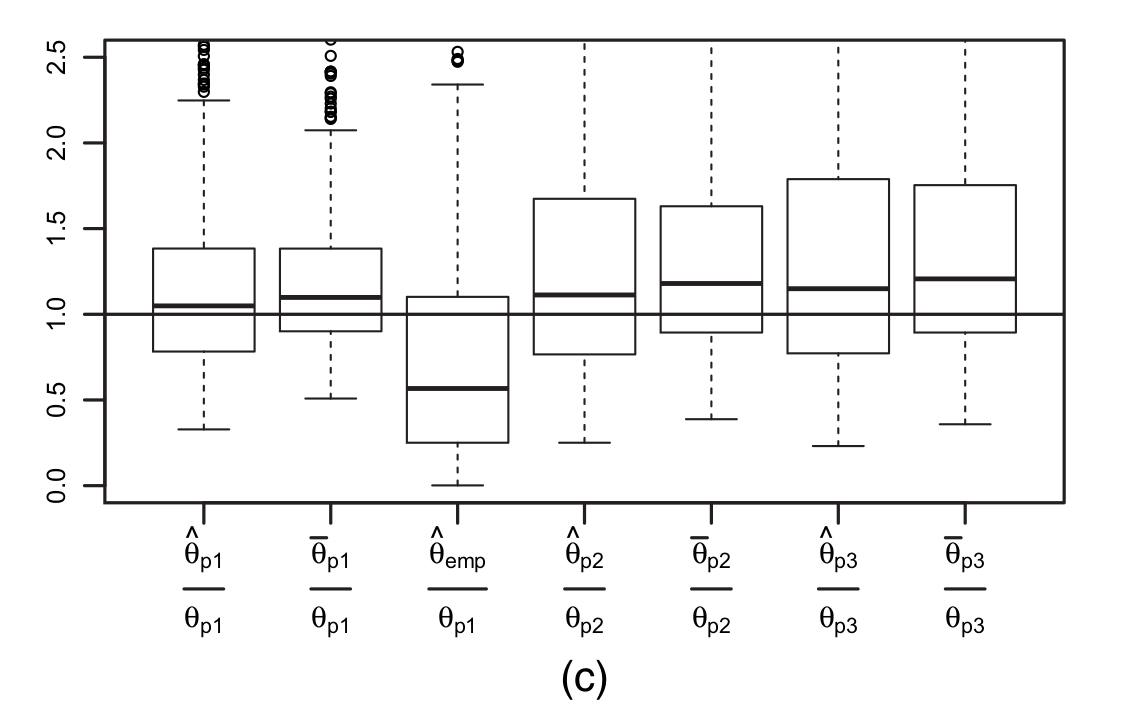
\includegraphics[width=0.8\textwidth]{c.png}

    

\end{frame}


\begin{frame}
    \frametitle{Simulation Distributions}
    We also investigate the performance of our estimator when our assumptions are partially
    violated.
    \begin{itemize}
    \item The transformed Cauchy distribution 3 is defined as
        $$
        (X, Y)=\left(\left|Z_{1}\right|^{0.7},\left|Z_{2}\right|\right).
        $$
$\gamma_1=0.7>1/2.$
    
    \item The second distribution is an asymptotically independent distribution defined as
        $$
        (X, Y)=\left(V_{1}+W_{1}, V_{2}+W_{2}\right),
        $$
        where $(V_1,V_2)$ follows the Student $t_3$-distribution and $W_1$ and $W_2$ are
        Pareto distributed with density $(25/2)(1+5x)^{-7/2}, x>0.$ Moreover, $(V_1,V_2), W_1$ and $W_2$ are independent. This does not satisfy condition (a).
    \end{itemize}
\end{frame}
\begin{frame}
    \frametitle{Boxplots of the estimates}
\begin{itemize}
    \item transformed Cauchy distribution 3.
\end{itemize}

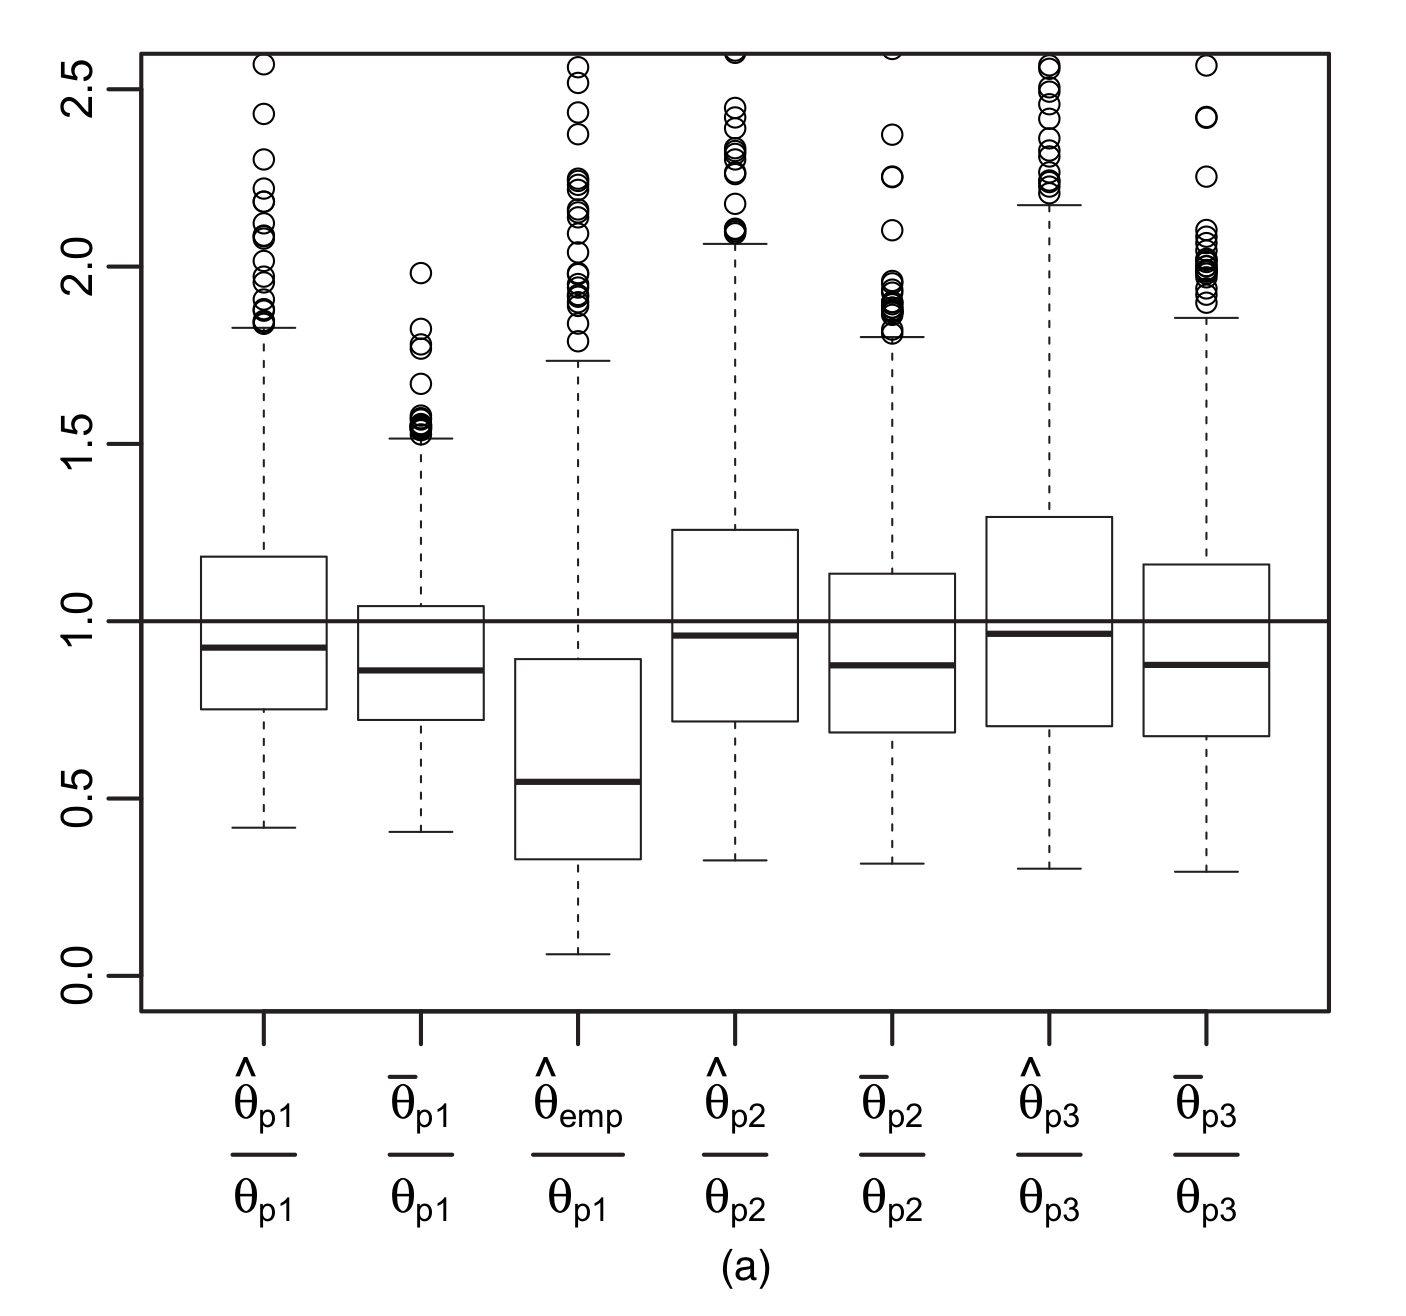
\includegraphics[width=0.6\textwidth]{2_a.png}


\end{frame}

\begin{frame}
    \frametitle{Boxplots of the estimates}
\begin{itemize}
    \item Asymptotically independent distribution.
\end{itemize}

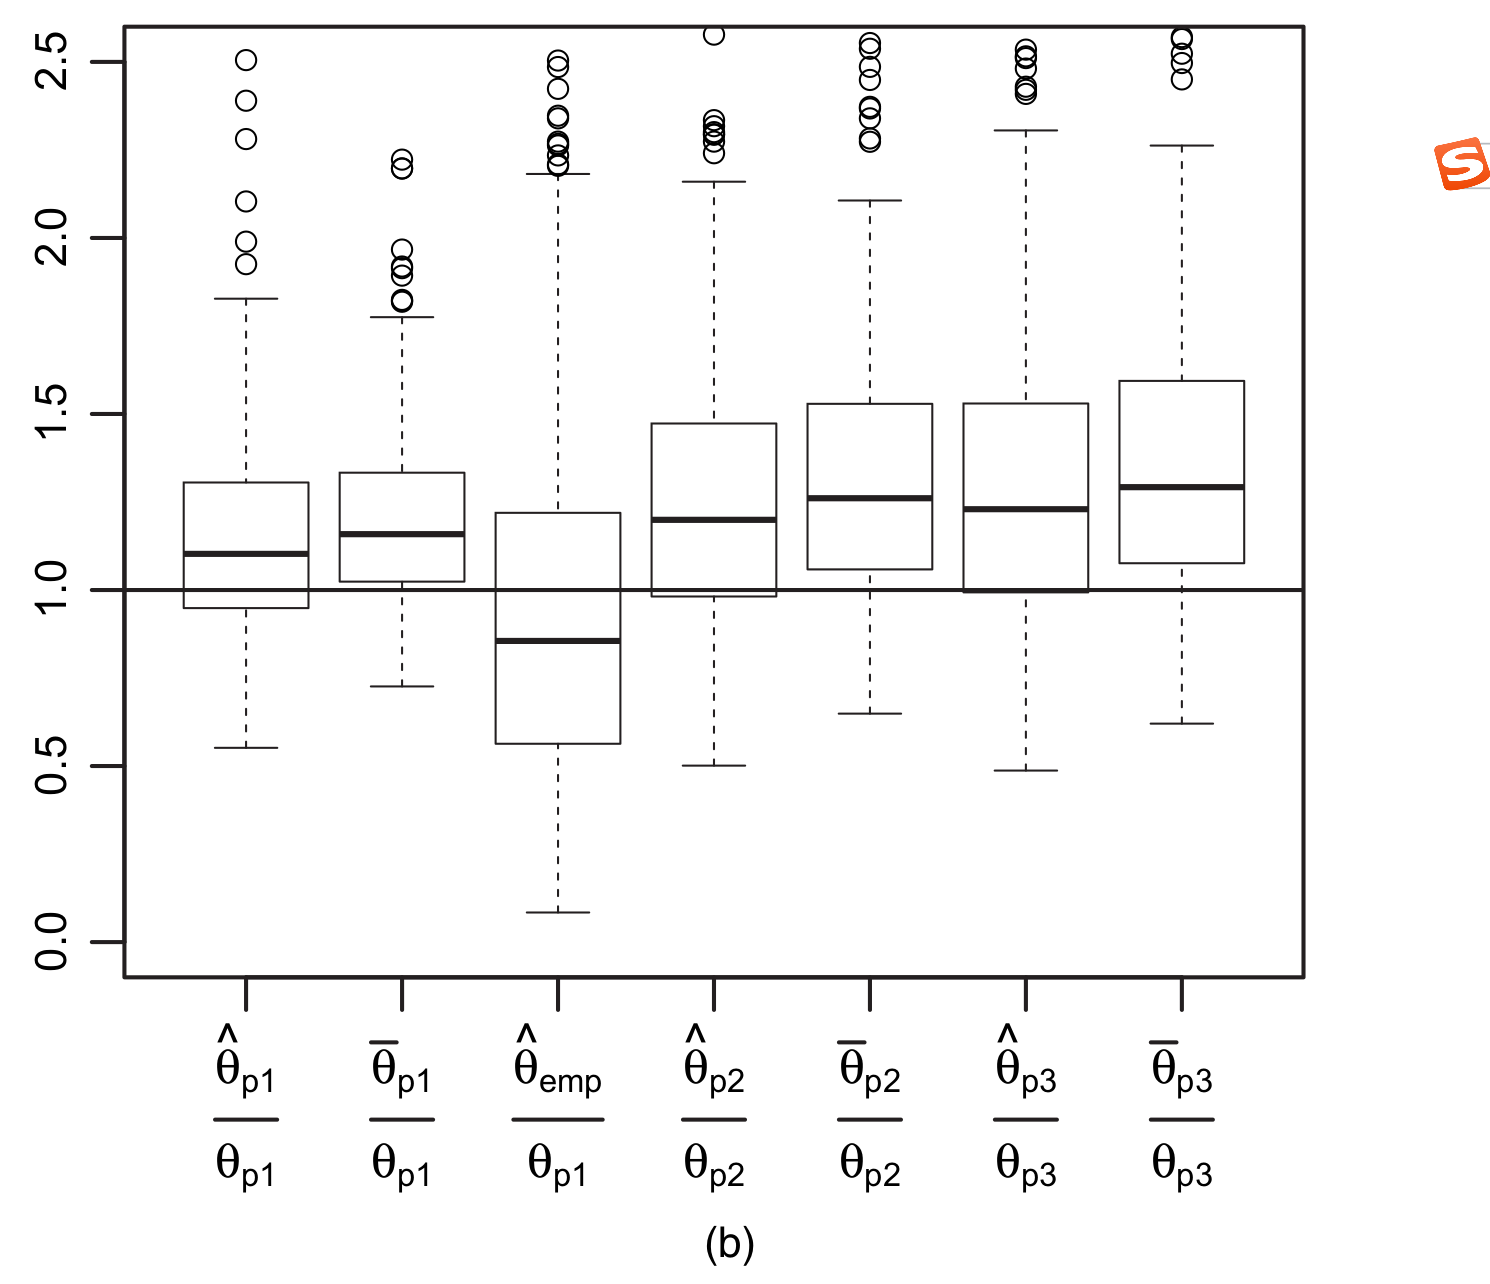
\includegraphics[width=0.6\textwidth]{2_b.png}


\end{frame}

\section{Application}

\begin{frame}
    \frametitle{Datasets}
\begin{itemize}
    \item We apply our estimation method to estimate the MES for financial institutions.
    \item We consider three large investment banks in the USA, namely Goldman Sachs, Morgan Stanley and T. Rowe Price. 
    \item Then, $X$ refers to each of these banks, $Y$ refers to the market index (value weighted index aggregating three markets: NYS, AE, NASDAQ).
    \item $n=2513$(daily loss) and $n=522$(weekly loss)
    \item  
    $p=1/n$ , which corresponds to a once-per-decade systemic event.
\end{itemize}
    
 


    

\end{frame}

\begin{frame}
    \frametitle{}
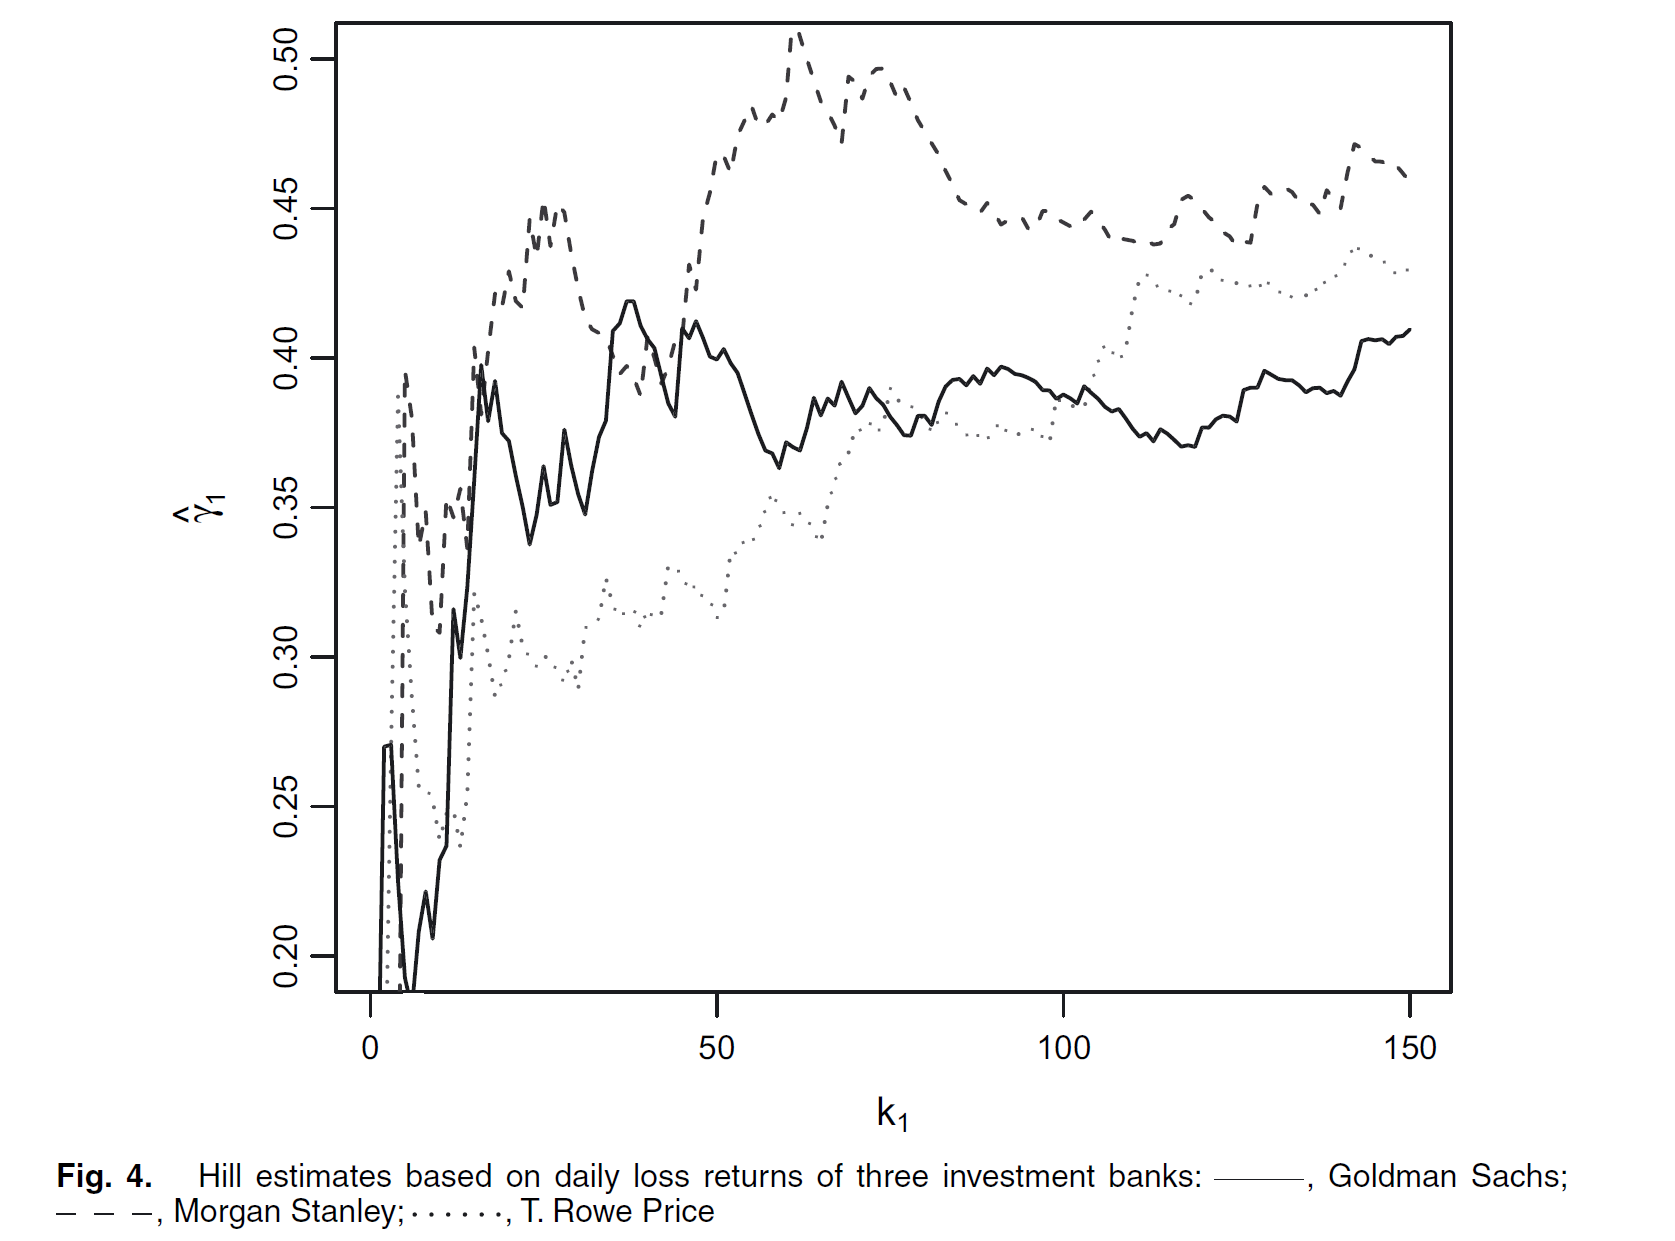
\includegraphics[width=1\textwidth]{Hill.png}
    

\end{frame}

\begin{frame}
    \frametitle{}
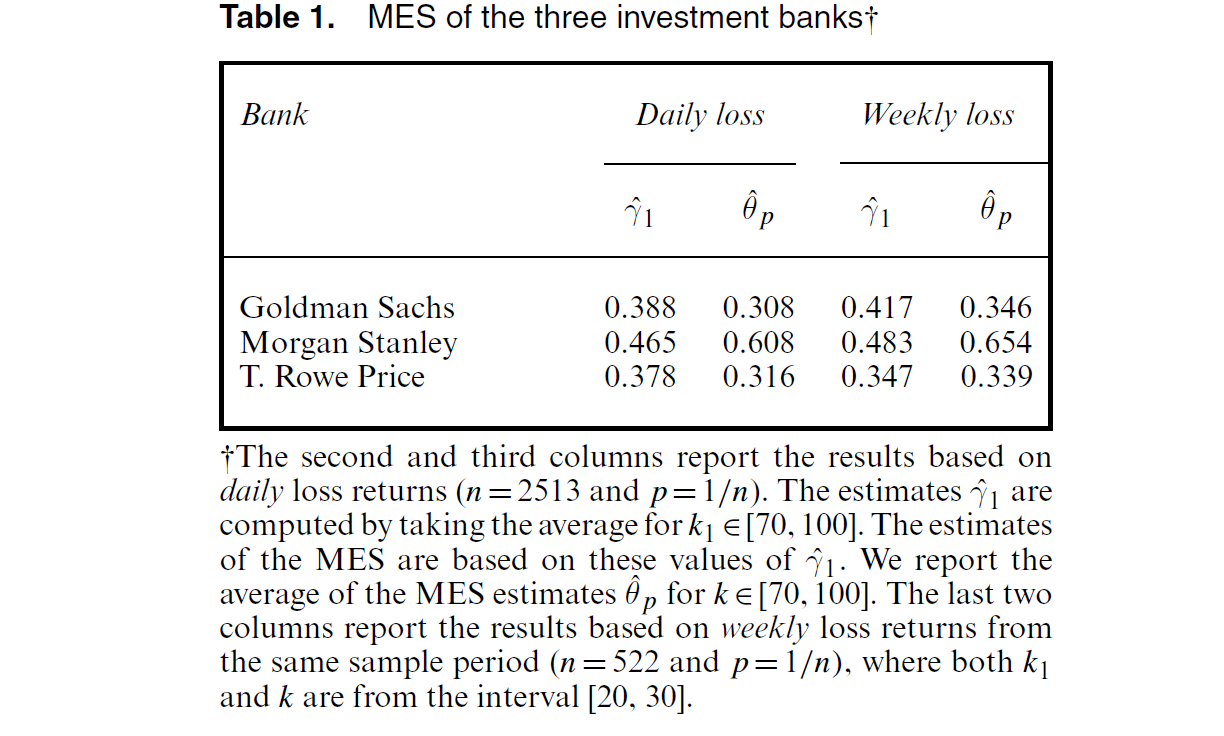
\includegraphics[width=1\textwidth]{Application.png}
    

\end{frame}


\end{document}